\documentclass[12pt,a4paper]{article}

\usepackage[utf8]{inputenc}
\usepackage[T2A]{fontenc}
\usepackage[ukrainian]{babel}
\usepackage{geometry}
\geometry{
    left=2cm,
    right=2cm,
    top=2cm,
    bottom=2cm
}

\usepackage[table]{xcolor}
\usepackage{amsmath}
\usepackage{graphicx}
\usepackage{subcaption}
\usepackage{multirow}
\usepackage{makecell}
\usepackage{pdflscape}
\usepackage{amsfonts}
\usepackage{array}
\newcolumntype{C}[1]{>{\centering\arraybackslash}m{#1}}

\usepackage[
  unicode,
  pdftitle={ІО-41, Давидчук А.М., Алгоритми та методи обчислень, Лабораторна робота №3},
  pdfauthor={Давидчук Артем},
  pdfsubject={Алгоритми та методи обчислень}
]{hyperref}

\usepackage{minted}

\usemintedstyle{vs}
\setminted{linenos, breaklines, frame=single, fontsize=\small}

\RecustomVerbatimCommand{\VerbatimInput}{VerbatimInput}{
    breaklines=true,
    breaksymbolleft={}
}

\begin{document}


    \begin{titlepage}

        \begin{center}
\includegraphics[width=0.7\textwidth]{../../../TITLES/letterhead.png}\end{center}

        \begin{center}
            \large Національний технічний університет України\\
            «Київський політехнічний інститут імені Ігоря Сікорського»\\[1em]
            Факультет інформатики та обчислювальної техніки\\
            Кафедра обчислювальної техніки
        \end{center}

        \vfill

        \begin{center}
            \textbf{\LARGE Алгоритми та методи обчислень}\\[2em]
            \textbf{\Large Лабораторна робота №3}\\[0.5em]
            «Інтерполяція функцій. Інтерполяційні многочлени»
        \end{center}

        \vfill

        \begin{flushright}
            Виконав: студент 2 курсу ФІОТ, гр. ІО-41\\
            \textit{Давидчук А. М.}\\
            Залікова книжка № 4106\\[1em]
            Перевірив: \textit{Порєв В.\,М.}
        \end{flushright}

        \vfill

        \begin{center}Київ --- 2026\end{center}

    \end{titlepage}

    \noindent
    \textbf{\underline{Тема:}} «Інтерполяція функцій. Інтерполяційні многочлени».

    \vspace{1em}

    \noindent
    \textbf{\underline{Мета:}} Ознайомлення з інтерполяційними формулами Лагранжа, Ньютона,
рекурентним співвідношенням Ейткена, методами оцінки похибки інтерполяції.

    \begin{center} \textbf{\Large Хід роботи} \end{center}

    Мій порядковий номер у списку групи: 6, звідси я маю інтерполювати таку функцію в таких межах за допомогою схеми Ейткена:

    \begin{figure}[h!]
        \centering
        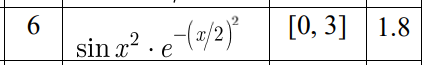
\includegraphics[width=0.6\linewidth]{media/ex.png}
        \caption{Варіант функції та способу інтерполяції}
    \end{figure}

    \noindent
    Також додатково я маю:

    \begin{enumerate}
        \item Передбачити в програмі оцінку похибки на основі порівняння значень, отриманих за допомогою інтерполяційних многочленів різного степеню;
        \item Оцінити розмитість оцінки похибки;
        \item Налагодити програму шляхом інтерполяції функції $\sin x$;
        \item Результат оцінки похибки представити у вигляді графіка.
    \end{enumerate}

    \vspace{1em}

    \noindent
    І так, опишемо словесно алгоритм методу Ейткена:

    \vspace{1em}

    Метод Ейткена є рекурентним способом обчислення значення інтерполяційного многочлена в заданій точці $x$. Основна перевага цього методу полягає в тому, що він дозволяє не виписувати явно весь інтерполяційний многочлен у алгебраїчному вигляді, а безпосередньо обчислювати його значення в потрібній точці.

    Метод базується на послідовному об'єднанні інтерполяційних многочленів нижчих степенів у многочлени вищих степенів. Спочатку беруться значення функції у вузлах, потім за ними будуються лінійні інтерполяції, далі квадратичні, кубічні і так далі, аж до многочлена найвищого степеня.

    Початкові значення задаються як
    $$
    P_{i,i}(x) = y_i = f(x_i), \quad i = 0,1,\dots,n.
    $$

    Далі для $i<j$ значення інтерполяційного многочлена обчислюється за рекурентною формулою:
    $$
    P_{i,j}(x)=
    \frac{(x-x_i)P_{i+1,j}(x)-(x-x_j)P_{i,j-1}(x)}{x_j-x_i}.
    $$

    Тут:
    \begin{itemize}
        \item $P_{i,j}(x)$ --- значення інтерполяційного многочлена, побудованого за вузлами $x_i, x_{i+1}, \dots, x_j$;
        \item $P_{i,i}(x)$ --- початкові значення, що дорівнюють значенням функції у вузлах;
        \item $P_{0,n}(x)$ --- остаточне значення інтерполяційного многочлена, побудованого за всіма вузлами.
    \end{itemize}

    Таким чином, результатом застосування методу Ейткена є число
    $$
    P_{0,n}(x),
    $$
    яке є наближеним значенням функції $f(x)$ у вибраній точці.

    Принцип методу Ейткена полягає у послідовному підвищенні степеня інтерполяційного многочлена. На нульовому кроці маємо лише значення функції у вузлах:
    $$
    P_{i,i}(x)=y_i.
    $$

    Потім із двох сусідніх значень будуються многочлени першого степеня:
    $$
    P_{i,i+1}(x).
    $$

    Далі з них будуються многочлени другого степеня:
    $$
    P_{i,i+2}(x),
    $$
    і так далі, поки не буде отримано
    $$
    P_{0,n}(x).
    $$

    Отже, метод має трикутну схему обчислень: кожен новий елемент таблиці визначається через два раніше знайдені елементи.

    \begin{enumerate}
        \item Задати відрізок інтерполювання та вибрати вузли
        $$
        x_0, x_1, \dots, x_n.
        $$

        \item Обчислити значення функції у вузлах:
        $$
        y_i = f(x_i), \quad i=0,1,\dots,n.
        $$

        \item Для заданої точки $x$ покласти початкові значення
        $$
        P_{i,i}(x)=y_i.
        $$

        \item Послідовно обчислювати значення
        $$
        P_{i,j}(x)
        $$
        за рекурентною формулою Ейткена, починаючи з многочленів першого степеня і закінчуючи многочленом степеня $n$.

        \item Остаточним результатом вважати значення
        $$
        P_{0,n}(x).
        $$

        \item Для аналізу точності порівняти значення, отримані для многочленів різних степенів.
    \end{enumerate}

    Якщо використовується $n+1$ вузлів інтерполяції, то будується інтерполяційний многочлен степеня не вище $n$. Наприклад:
    \begin{itemize}
        \item за 2 вузлами будується многочлен 1-го степеня;
        \item за 3 вузлами --- многочлен 2-го степеня;
        \item за 11 вузлами --- многочлен 10-го степеня.
    \end{itemize}

    Тому в таблиці обчислень величина $n$ зазвичай означає саме степінь інтерполяційного многочлена.

    Оскільки інтерполяційний многочлен лише наближує функцію між вузлами, виникає похибка інтерполяції. Її можна визначити як різницю між точним значенням функції та значенням інтерполяційного многочлена:
    $$
    R_n(x)=f(x)-P_n(x).
    $$

    Абсолютна похибка дорівнює
    $$
    |R_n(x)| = |f(x)-P_n(x)|.
    $$

    Якщо точне значення функції відоме, то це є найзручнішою формулою для обчислення реальної похибки.

    Для інтерполяційного многочлена степеня $n$ теоретична похибка має вигляд
    $$
    R_n(x)=
    \frac{f^{(n+1)}(\xi)}{(n+1)!}
    (x-x_0)(x-x_1)\cdots(x-x_n),
    $$
    де $\xi$ --- деяка точка з проміжку, що містить вузли інтерполяції та точку $x$.

    Ця формула показує, що величина похибки залежить від:
    \begin{itemize}
        \item похідної порядку $n+1$ від функції;
        \item кількості та розташування вузлів;
        \item положення точки $x$ відносно вузлів.
    \end{itemize}

    На практиці ця формула не завжди зручна для числового обчислення, оскільки значення $\xi$ невідоме.

    У чисельних методах часто використовують практичну оцінку похибки на основі порівняння результатів, отриманих для многочленів сусідніх степенів:
    $$
    \varepsilon_n(x)\approx |P_n(x)-P_{n-1}(x)|.
    $$

    Така оцінка базується на тому, що при збільшенні степеня інтерполяційного многочлена наближення має стабілізуватися, а різниця між сусідніми наближеннями стає малою.

    Якщо
    $$
    |P_n(x)-P_{n-1}(x)|
    $$
    мале, то це свідчить про те, що значення інтерполяції вже майже не змінюється і наближення є достатньо точним.

    Крім абсолютної похибки, інколи розглядають відносну похибку:
    $$
    \delta_n(x)=\frac{|f(x)-P_n(x)|}{|f(x)|},
    \quad f(x)\neq 0.
    $$

    У відсотках вона записується так:
    $$
    \delta_n(x)\cdot 100\%.
    $$

    Відносна похибка показує, наскільки велика помилка порівняно з самим значенням функції.

    Похибка інтерполяції може збільшуватися з таких причин:
    \begin{itemize}
        \item функція має складну поведінку на відрізку;
        \item вузли розташовані невдало;
        \item точка $x$ знаходиться поблизу краю інтервалу;
        \item використовується многочлен занадто високого степеня, що може призводити до осциляцій.
    \end{itemize}

    Тому на практиці важливо не лише побудувати інтерполяцію, а й оцінити її точність.

    \newpage

    \noindent
    Блок-схема алгоритму методу Ейткена:

    \begin{figure}[h!]
        \centering
        \includegraphics[width=0.65\linewidth]{media/block.drawio3_cropped.pdf}
        \caption{Блок-схема методу Ейткена}
    \end{figure}

    \newpage

    Для реалізації алгоритмів та GUI середовища я використовуватиму мову програмування Python і інструмент Tkinter та бібліотеку customtkinter.

    \vspace{1em}

    \noindent
    \textbf{\underline{Програмний код для реалізації метода Ейткена для інтерполювання}}:

    \vspace{1em}

    \noindent
    \underline{(\texttt{app.py})}

    \begin{minted}{python3}
from src.gui import main

if __name__ == "__main__":

    main()
    \end{minted}

    \noindent
    \underline{(\texttt{src/aitken.py})}

    \begin{minted}{python3}
from __future__ import annotations

def build_nodes(a: float, b: float, parts: int = 10) -> list[float]:
    h = (b - a) / parts
    return [a + i * h for i in range(parts + 1)]

def calculate_function_values(func, x_nodes: list[float]) -> list[float]:
    return [func(x) for x in x_nodes]

def interpolate_full(x_nodes: list[float], y_nodes: list[float], x: float) -> float:
    table = aitken_table(x_nodes, y_nodes, x)
    return table[0][len(x_nodes) - 1]

def aitken_table(x_nodes: list[float], y_nodes: list[float], x: float) -> list[list[float]]:
    n = len(x_nodes)
    p = [[0.0 for _ in range(n)] for _ in range(n)]

    for i in range(n):
        p[i][0] = y_nodes[i]

    for j in range(1, n):
        for i in range(n - j):
            denominator = x_nodes[i + j] - x_nodes[i]
            if abs(denominator) < 1e-15:
                raise ZeroDivisionError("Zero denominator in Aitken scheme.")
            p[i][j] = (
                (x - x_nodes[i]) * p[i + 1][j - 1]
                - (x - x_nodes[i + j]) * p[i][j - 1]
            ) / denominator

    return p

def aitken_by_degree(x_nodes: list[float], y_nodes: list[float], x: float) -> list[float]:
    approximations: list[float] = []

    for degree in range(len(x_nodes)):
        sub_x = x_nodes[: degree + 1]
        sub_y = y_nodes[: degree + 1]
        table = aitken_table(sub_x, sub_y, x)
        approximations.append(table[0][degree])

    return approximations
    \end{minted}

    \noindent
    \underline{(\texttt{src/error\_analysis.py})}

    \begin{minted}{python3}
from __future__ import annotations

from src.aitken import aitken_by_degree
from src.models import ErrorRow

def compute_error_rows(func, x_nodes: list[float], y_nodes: list[float], x_value: float) -> tuple[float, list[ErrorRow]]:
    true_value = func(x_value)
    approximations = aitken_by_degree(x_nodes, y_nodes, x_value)

    rows: list[ErrorRow] = []
    for degree, approx in enumerate(approximations):
        estimate = None if degree == 0 else abs(approximations[degree] - approximations[degree - 1])
        actual_error = abs(true_value - approx)
        rows.append(
            ErrorRow(
                degree=degree,
                approximation=approx,
                estimate=estimate,
                actual_error=actual_error,
            )
        )
    return true_value, rows
    \end{minted}

    \noindent
    \underline{(\texttt{src/functions.py})}

    \begin{minted}{python3}
from __future__ import annotations

import math
from typing import Callable

def target_function(x: float) -> float:
    return math.sin(x ** 2) * math.exp(-((x / 2) ** 2))

def test_function(x: float) -> float:
    return math.sin(x)

def get_function_by_name(name: str) -> tuple[Callable[[float], float], str]:
    if name == "test":
        return test_function, "sin(x)"
    return target_function, "sin(x^2) * exp(-(x/2)^2)"
    \end{minted}

    \noindent
    \underline{(\texttt{src/graph\_build.py})}

    \begin{minted}{python3}
from __future__ import annotations

from matplotlib.figure import Figure

from src.aitken import interpolate_full


def build_interpolation_figure(
    func,
    x_nodes: list[float],
    y_nodes: list[float],
    a: float,
    b: float,
    x_value: float,
    plot_points: int,
) -> Figure:
    x_dense = [a + (b - a) * i / (plot_points - 1) for i in range(plot_points)]
    y_true = [func(x) for x in x_dense]
    y_interp = [interpolate_full(x_nodes, y_nodes, x) for x in x_dense]
    y_error = [abs(y1 - y2) for y1, y2 in zip(y_true, y_interp)]

    true_at_x = func(x_value)
    interp_at_x = interpolate_full(x_nodes, y_nodes, x_value)

    fig = Figure(figsize=(8.2, 5.8), dpi=100)
    ax = fig.add_subplot(111)

    ax.plot(x_dense, y_true, label="f(x)")
    ax.plot(x_dense, y_interp, label="Aitken interpolation")
    ax.plot(x_dense, y_error, label="|f(x)-P(x)|")
    ax.scatter(x_nodes, y_nodes, label="Nodes")
    ax.scatter([x_value], [true_at_x], label="f(x*)")
    ax.scatter([x_value], [interp_at_x], label="P(x*)")

    ax.set_title("Aitken interpolation graph")
    ax.set_xlabel("x")
    ax.set_ylabel("y")
    ax.grid(True)
    ax.legend()
    fig.tight_layout()

    return fig
    \end{minted}

    \noindent
    \underline{(\texttt{src/gui.py})}

    \begin{minted}{python3}
from __future__ import annotations

import tkinter as tk
from dataclasses import dataclass
from tkinter import filedialog, ttk

import customtkinter as ctk
from matplotlib.backends.backend_tkagg import FigureCanvasTkAgg

from src.aitken import build_nodes, calculate_function_values
from src.error_analysis import compute_error_rows
from src.functions import get_function_by_name
from src.graph_build import build_interpolation_figure
from src.io_utils import load_json_config
from src.models import PageConfig
from src.report import build_full_report, build_short_result
from src.theme import MAIN_THEME


@dataclass
class InterpolationState:
    function_name: str = "target"
    function_title: str = "sin(x^2) * exp(-(x/2)^2)"
    a: float = 0.0
    b: float = 3.0
    x_value: float = 1.5
    parts: int = 10
    plot_points: int = 400
    x_nodes: list[float] | None = None
    y_nodes: list[float] | None = None
    true_value: float | None = None
    rows: list | None = None
    report: str = ""


class BasePage(ctk.CTkFrame):
    def __init__(
        self,
        master: ctk.CTkFrame,
        page_config: PageConfig,
        fonts: dict[str, ctk.CTkFont],
    ) -> None:
        super().__init__(master, corner_radius=0)
        self.page_config = page_config
        self.fonts = fonts
        self.grid_columnconfigure(0, weight=1)

    def apply_theme(self, palette: dict[str, str]) -> None:
        self.configure(fg_color=palette["bg"])


class MainPage(BasePage):
    def __init__(
        self,
        master: ctk.CTkFrame,
        page_config: PageConfig,
        fonts: dict[str, ctk.CTkFont],
        app_state: InterpolationState,
    ) -> None:
        super().__init__(master, page_config, fonts)
        self.app_state = app_state

        self.result_var = tk.StringVar(value="Ready")
        self.error_var = tk.StringVar(value="")

        self.grid_rowconfigure(3, weight=1)
        self.grid_columnconfigure(0, weight=1)

        self._build_header()
        self._build_form()
        self._build_actions()
        self._build_output()
        self.reset_defaults()

    def _build_header(self) -> None:
        self.header_card = ctk.CTkFrame(self, corner_radius=14, border_width=1)
        self.header_card.grid(row=0, column=0, sticky="ew", pady=(0, 14))
        self.header_card.grid_columnconfigure(0, weight=1)

        self.title_label = ctk.CTkLabel(
            self.header_card,
            text=self.page_config.title,
            anchor="w",
            font=self.fonts["title"],
        )
        self.title_label.grid(row=0, column=0, sticky="ew", padx=20, pady=(14, 4))

        self.subtitle_label = ctk.CTkLabel(
            self.header_card,
            text=self.page_config.subtitle,
            anchor="w",
            font=self.fonts["subtitle"],
        )
        self.subtitle_label.grid(row=1, column=0, sticky="ew", padx=20, pady=(0, 12))

    def _build_form(self) -> None:
        self.form_card = ctk.CTkFrame(self, corner_radius=14, border_width=1)
        self.form_card.grid(row=1, column=0, sticky="ew", pady=(0, 14))
        self.form_card.grid_columnconfigure((0, 1), weight=1)

        self.function_label = ctk.CTkLabel(
            self.form_card,
            text="Function:",
            anchor="w",
            font=self.fonts["label"],
        )
        self.function_label.grid(row=0, column=0, sticky="w", padx=20, pady=(14, 6))

        self.function_menu = ctk.CTkOptionMenu(
            self.form_card,
            values=["target", "test"],
            font=self.fonts["body"],
            command=self._on_function_change,
        )
        self.function_menu.grid(row=1, column=0, sticky="ew", padx=(20, 8), pady=(0, 12))

        self.load_button = ctk.CTkButton(
            self.form_card,
            text="Load JSON",
            height=40,
            corner_radius=11,
            font=self.fonts["button"],
            command=self.load_json,
        )
        self.load_button.grid(row=1, column=1, sticky="ew", padx=(8, 20), pady=(0, 12))

        self.entry_a = self._build_labeled_entry(self.form_card, 2, 0, "a:")
        self.entry_b = self._build_labeled_entry(self.form_card, 2, 1, "b:")
        self.entry_x = self._build_labeled_entry(self.form_card, 4, 0, "x:")
        self.entry_parts = self._build_labeled_entry(self.form_card, 4, 1, "Parts:")
        self.entry_plot_points = self._build_labeled_entry(self.form_card, 6, 0, "Plot points:")

    def _build_labeled_entry(
        self,
        parent: ctk.CTkFrame,
        row: int,
        column: int,
        label_text: str,
    ) -> ctk.CTkEntry:
        label = ctk.CTkLabel(
            parent,
            text=label_text,
            anchor="w",
            font=self.fonts["label"],
        )
        label.grid(row=row, column=column, sticky="w", padx=20, pady=(0, 6))

        entry = ctk.CTkEntry(
            parent,
            height=40,
            corner_radius=10,
            font=self.fonts["body"],
        )
        entry.grid(row=row + 1, column=column, sticky="ew", padx=20, pady=(0, 12))
        return entry

    def _build_actions(self) -> None:
        self.actions = ctk.CTkFrame(self, fg_color="transparent")
        self.actions.grid(row=2, column=0, sticky="ew", pady=(0, 10))
        self.actions.grid_columnconfigure((0, 1, 2), weight=1)

        self.compute_button = ctk.CTkButton(
            self.actions,
            text="Compute",
            height=40,
            corner_radius=11,
            font=self.fonts["button"],
            command=self.compute,
        )
        self.compute_button.grid(row=0, column=0, sticky="ew", padx=(0, 7))

        self.save_button = ctk.CTkButton(
            self.actions,
            text="Save Report",
            height=40,
            corner_radius=11,
            font=self.fonts["button"],
            command=self.save_report,
        )
        self.save_button.grid(row=0, column=1, sticky="ew", padx=7)

        self.clear_button = ctk.CTkButton(
            self.actions,
            text="Clear",
            height=40,
            corner_radius=11,
            font=self.fonts["button"],
            command=self.clear_all,
        )
        self.clear_button.grid(row=0, column=2, sticky="ew", padx=(7, 0))

    def _build_output(self) -> None:
        self.output_card = ctk.CTkFrame(self, corner_radius=14, border_width=1)
        self.output_card.grid(row=3, column=0, sticky="nsew")
        self.output_card.grid_columnconfigure(0, weight=1)
        self.output_card.grid_rowconfigure(4, weight=1)

        self.result_title = ctk.CTkLabel(
            self.output_card,
            text="Result",
            anchor="w",
            font=self.fonts["label"],
        )
        self.result_title.grid(row=0, column=0, sticky="ew", padx=20, pady=(14, 6))

        self.result_label = ctk.CTkLabel(
            self.output_card,
            textvariable=self.result_var,
            anchor="w",
            justify="left",
            wraplength=860,
            font=self.fonts["result"],
        )
        self.result_label.grid(row=1, column=0, sticky="ew", padx=20, pady=(0, 8))

        self.error_label = ctk.CTkLabel(
            self.output_card,
            textvariable=self.error_var,
            anchor="w",
            justify="left",
            wraplength=860,
            font=self.fonts["body"],
        )
        self.error_label.grid(row=2, column=0, sticky="ew", padx=20, pady=(0, 10))

        self.table_title = ctk.CTkLabel(
            self.output_card,
            text="Table",
            anchor="w",
            font=self.fonts["label"],
        )
        self.table_title.grid(row=3, column=0, sticky="ew", padx=20, pady=(0, 6))

        self.table_frame = tk.Frame(self.output_card, bg="#090909")
        self.table_frame.grid(row=4, column=0, sticky="nsew", padx=20, pady=(0, 14))
        self.table_frame.grid_rowconfigure(0, weight=1)
        self.table_frame.grid_columnconfigure(0, weight=1)

        columns = ("degree", "approximation", "estimate", "actual_error")
        self.results_table = ttk.Treeview(
            self.table_frame,
            columns=columns,
            show="headings",
            height=11,
        )

        self.results_table.heading("degree", text="n")
        self.results_table.heading("approximation", text="P_n(x)")
        self.results_table.heading("estimate", text="|P_n - P_(n-1)|")
        self.results_table.heading("actual_error", text="|f(x) - P_n(x)|")

        self.results_table.column("degree", width=70, anchor="center")
        self.results_table.column("approximation", width=190, anchor="center")
        self.results_table.column("estimate", width=190, anchor="center")
        self.results_table.column("actual_error", width=190, anchor="center")

        self.table_scrollbar = ttk.Scrollbar(
            self.table_frame,
            orient="vertical",
            command=self.results_table.yview,
        )
        self.results_table.configure(yscrollcommand=self.table_scrollbar.set)

        self.results_table.grid(row=0, column=0, sticky="nsew")
        self.table_scrollbar.grid(row=0, column=1, sticky="ns")

    def _fill_table(self, rows) -> None:
        for item in self.results_table.get_children():
            self.results_table.delete(item)

        for row in rows:
            estimate_text = "-" if row.estimate is None else f"{row.estimate:.10f}"
            self.results_table.insert(
                "",
                "end",
                values=(
                    row.degree,
                    f"{row.approximation:.10f}",
                    estimate_text,
                    f"{row.actual_error:.10f}",
                ),
            )

    def _on_function_change(self, choice: str) -> None:
        if choice == "test":
            self.entry_a.delete(0, tk.END)
            self.entry_a.insert(0, "0")
            self.entry_b.delete(0, tk.END)
            self.entry_b.insert(0, "3.1415926535")
            self.entry_x.delete(0, tk.END)
            self.entry_x.insert(0, "1.0")
            self.entry_parts.delete(0, tk.END)
            self.entry_parts.insert(0, "10")
            self.entry_plot_points.delete(0, tk.END)
            self.entry_plot_points.insert(0, "400")
        else:
            self.entry_a.delete(0, tk.END)
            self.entry_a.insert(0, "0")
            self.entry_b.delete(0, tk.END)
            self.entry_b.insert(0, "3")
            self.entry_x.delete(0, tk.END)
            self.entry_x.insert(0, "1.5")
            self.entry_parts.delete(0, tk.END)
            self.entry_parts.insert(0, "10")
            self.entry_plot_points.delete(0, tk.END)
            self.entry_plot_points.insert(0, "400")

    def load_json(self) -> None:
        path = filedialog.askopenfilename(
            title="Select JSON file",
            filetypes=[("JSON files", "*.json"), ("All files", "*.*")],
        )
        if not path:
            return

        try:
            loaded = load_json_config(path)

            function_name = str(loaded.get("function", "target"))
            self.function_menu.set(function_name)

            self.entry_a.delete(0, tk.END)
            self.entry_a.insert(0, str(loaded.get("a", 0)))

            self.entry_b.delete(0, tk.END)
            self.entry_b.insert(0, str(loaded.get("b", 3)))

            self.entry_x.delete(0, tk.END)
            self.entry_x.insert(0, str(loaded.get("x_value", 1.5)))

            self.entry_parts.delete(0, tk.END)
            self.entry_parts.insert(0, str(loaded.get("parts", 10)))

            self.entry_plot_points.delete(0, tk.END)
            self.entry_plot_points.insert(0, str(loaded.get("plot_points", 400)))

            self.result_var.set("JSON loaded. Press Compute.")
            self.error_var.set("")
        except Exception as exc:
            self.result_var.set("No result")
            self.error_var.set(f"Error: {exc}")

    def _parse_input(self) -> tuple[str, float, float, float, int, int]:
        function_name = self.function_menu.get()
        a = float(self.entry_a.get().strip())
        b = float(self.entry_b.get().strip())
        x_value = float(self.entry_x.get().strip())
        parts = int(self.entry_parts.get().strip())
        plot_points = int(self.entry_plot_points.get().strip())

        if b <= a:
            raise ValueError("Потрібно, щоб b > a.")
        if parts < 1:
            raise ValueError("Кількість частин має бути не меншою за 1.")
        if plot_points < 50:
            raise ValueError("Кількість точок для графіка має бути не меншою за 50.")
        if not (a <= x_value <= b):
            raise ValueError("Точка x повинна належати відрізку [a, b].")

        return function_name, a, b, x_value, parts, plot_points

    def compute(self) -> None:
        try:
            function_name, a, b, x_value, parts, plot_points = self._parse_input()
            func, function_title = get_function_by_name(function_name)

            x_nodes = build_nodes(a, b, parts)
            y_nodes = calculate_function_values(func, x_nodes)
            true_value, rows = compute_error_rows(func, x_nodes, y_nodes, x_value)

            report = build_full_report(
                func_name=function_title,
                a=a,
                b=b,
                x_value=x_value,
                x_nodes=x_nodes,
                y_nodes=y_nodes,
                rows=rows,
                true_value=true_value,
            )

            self.app_state.function_name = function_name
            self.app_state.function_title = function_title
            self.app_state.a = a
            self.app_state.b = b
            self.app_state.x_value = x_value
            self.app_state.parts = parts
            self.app_state.plot_points = plot_points
            self.app_state.x_nodes = x_nodes
            self.app_state.y_nodes = y_nodes
            self.app_state.true_value = true_value
            self.app_state.rows = rows
            self.app_state.report = report

            self.result_var.set(build_short_result(rows, true_value))
            self.error_var.set("")
            self._fill_table(rows)
        except Exception as exc:
            self.result_var.set("No result")
            self.error_var.set(f"Error: {exc}")

    def save_report(self) -> None:
        if not self.app_state.report.strip():
            self.result_var.set("No result")
            self.error_var.set("Error: Спочатку виконай обчислення.")
            return

        path = filedialog.asksaveasfilename(
            title="Save report",
            defaultextension=".txt",
            filetypes=[("Text files", "*.txt"), ("All files", "*.*")],
        )
        if not path:
            return

        try:
            with open(path, "w", encoding="utf-8") as file:
                file.write(self.app_state.report)
            self.error_var.set("")
        except Exception as exc:
            self.error_var.set(f"Error: {exc}")

    def clear_all(self) -> None:
        self.reset_defaults()

    def reset_defaults(self) -> None:
        self.function_menu.set("target")

        self.entry_a.delete(0, tk.END)
        self.entry_a.insert(0, "0")

        self.entry_b.delete(0, tk.END)
        self.entry_b.insert(0, "3")

        self.entry_x.delete(0, tk.END)
        self.entry_x.insert(0, "1.5")

        self.entry_parts.delete(0, tk.END)
        self.entry_parts.insert(0, "10")

        self.entry_plot_points.delete(0, tk.END)
        self.entry_plot_points.insert(0, "400")

        self.result_var.set("Ready")
        self.error_var.set("")

        for item in self.results_table.get_children():
            self.results_table.delete(item)

        self.app_state.function_name = "target"
        self.app_state.function_title = "sin(x^2) * exp(-(x/2)^2)"
        self.app_state.a = 0.0
        self.app_state.b = 3.0
        self.app_state.x_value = 1.5
        self.app_state.parts = 10
        self.app_state.plot_points = 400
        self.app_state.x_nodes = None
        self.app_state.y_nodes = None
        self.app_state.true_value = None
        self.app_state.rows = None
        self.app_state.report = ""

    def apply_theme(self, palette: dict[str, str]) -> None:
        super().apply_theme(palette)

        for card in (self.header_card, self.form_card, self.output_card):
            card.configure(
                fg_color=palette["panel"],
                border_color=palette["surface_soft"],
            )

        self.title_label.configure(text_color=palette["text"])
        self.subtitle_label.configure(text_color=palette["muted"])
        self.function_label.configure(text_color=palette["muted"])

        for entry in (
            self.entry_a,
            self.entry_b,
            self.entry_x,
            self.entry_parts,
            self.entry_plot_points,
        ):
            entry.configure(
                fg_color=palette["surface"],
                border_color=palette["surface_soft"],
                text_color=palette["text"],
            )

        self.function_menu.configure(
            fg_color=palette["segment_active"],
            button_color=palette["segment"],
            button_hover_color=palette["segment_hover"],
            text_color=palette["text"],
        )

        self.compute_button.configure(
            fg_color=palette["accent"],
            hover_color=palette["accent_hover"],
            text_color=palette["accent_text"],
        )
        self.load_button.configure(
            fg_color=palette["segment"],
            hover_color=palette["segment_hover"],
            text_color=palette["text"],
        )
        self.save_button.configure(
            fg_color=palette["segment"],
            hover_color=palette["segment_hover"],
            text_color=palette["text"],
        )
        self.clear_button.configure(
            fg_color=palette["segment"],
            hover_color=palette["segment_hover"],
            text_color=palette["text"],
        )

        self.result_title.configure(text_color=palette["muted"])
        self.table_title.configure(text_color=palette["muted"])
        self.result_label.configure(text_color=palette["text"])
        self.error_label.configure(text_color=palette["error"])

        style = ttk.Style()
        style.theme_use("default")

        style.configure(
            "Treeview",
            background="#111111",
            foreground="#F5F7FA",
            fieldbackground="#111111",
            rowheight=28,
            bordercolor="#1B1B1B",
            borderwidth=1,
        )
        style.configure(
            "Treeview.Heading",
            background="#131313",
            foreground="#F5F7FA",
            relief="flat",
        )
        style.map(
            "Treeview",
            background=[("selected", "#1F2D3C")],
            foreground=[("selected", "#F5F7FA")],
        )


class GraphPage(BasePage):
    def __init__(
        self,
        master: ctk.CTkFrame,
        page_config: PageConfig,
        fonts: dict[str, ctk.CTkFont],
        app_state: InterpolationState,
    ) -> None:
        super().__init__(master, page_config, fonts)
        self.app_state = app_state

        self.status_var = tk.StringVar(value="Ready to build graph")
        self.error_var = tk.StringVar(value="")
        self.canvas: FigureCanvasTkAgg | None = None

        self.grid_rowconfigure(3, weight=1)

        self._build_header()
        self._build_controls()
        self._build_output()
        self._build_plot_area()

    def _build_header(self) -> None:
        self.header_card = ctk.CTkFrame(self, corner_radius=14, border_width=1)
        self.header_card.grid(row=0, column=0, sticky="ew", pady=(0, 14))
        self.header_card.grid_columnconfigure(0, weight=1)

        self.title_label = ctk.CTkLabel(
            self.header_card,
            text=self.page_config.title,
            anchor="w",
            font=self.fonts["title"],
        )
        self.title_label.grid(row=0, column=0, sticky="ew", padx=20, pady=(14, 4))

        self.subtitle_label = ctk.CTkLabel(
            self.header_card,
            text=self.page_config.subtitle,
            anchor="w",
            font=self.fonts["subtitle"],
        )
        self.subtitle_label.grid(row=1, column=0, sticky="ew", padx=20, pady=(0, 12))

    def _build_controls(self) -> None:
        self.controls_card = ctk.CTkFrame(self, corner_radius=14, border_width=1)
        self.controls_card.grid(row=1, column=0, sticky="ew", pady=(0, 14))
        self.controls_card.grid_columnconfigure(0, weight=1)

        self.info_label = ctk.CTkLabel(
            self.controls_card,
            text=(
                "Побудова графіка функції, повної інтерполяції за схемою Ейткена "
                "та абсолютної похибки |f(x)-P(x)|."
            ),
            anchor="w",
            justify="left",
            wraplength=860,
            font=self.fonts["body"],
        )
        self.info_label.grid(row=0, column=0, sticky="ew", padx=20, pady=(14, 12))

        self.build_button = ctk.CTkButton(
            self.controls_card,
            text="Build Graph",
            height=40,
            corner_radius=11,
            font=self.fonts["button"],
            command=self.build_graph,
        )
        self.build_button.grid(row=1, column=0, sticky="ew", padx=20, pady=(0, 14))

    def _build_output(self) -> None:
        self.output_card = ctk.CTkFrame(self, corner_radius=14, border_width=1)
        self.output_card.grid(row=2, column=0, sticky="ew")
        self.output_card.grid_columnconfigure(0, weight=1)

        self.status_title = ctk.CTkLabel(
            self.output_card,
            text="Status",
            anchor="w",
            font=self.fonts["label"],
        )
        self.status_title.grid(row=0, column=0, sticky="ew", padx=20, pady=(14, 6))

        self.status_label = ctk.CTkLabel(
            self.output_card,
            textvariable=self.status_var,
            anchor="w",
            justify="left",
            wraplength=860,
            font=self.fonts["result"],
        )
        self.status_label.grid(row=1, column=0, sticky="ew", padx=20, pady=(0, 8))

        self.error_label = ctk.CTkLabel(
            self.output_card,
            textvariable=self.error_var,
            anchor="w",
            justify="left",
            wraplength=860,
            font=self.fonts["body"],
        )
        self.error_label.grid(row=2, column=0, sticky="ew", padx=20, pady=(0, 14))

    def _build_plot_area(self) -> None:
        self.plot_card = ctk.CTkFrame(self, corner_radius=14, border_width=1)
        self.plot_card.grid(row=3, column=0, sticky="nsew", pady=(14, 0))
        self.plot_card.grid_columnconfigure(0, weight=1)
        self.plot_card.grid_rowconfigure(0, weight=1)

        self.plot_container = ctk.CTkFrame(self.plot_card, fg_color="transparent")
        self.plot_container.grid(row=0, column=0, sticky="nsew", padx=12, pady=12)
        self.plot_container.grid_columnconfigure(0, weight=1)
        self.plot_container.grid_rowconfigure(0, weight=1)

    def build_graph(self) -> None:
        try:
            if self.app_state.x_nodes is None or self.app_state.y_nodes is None:
                raise ValueError("Спочатку виконай обчислення на сторінці Main.")

            self.status_var.set("Building graph...")
            self.error_var.set("")
            self.update_idletasks()

            func, _ = get_function_by_name(self.app_state.function_name)
            fig = build_interpolation_figure(
                func=func,
                x_nodes=self.app_state.x_nodes,
                y_nodes=self.app_state.y_nodes,
                a=self.app_state.a,
                b=self.app_state.b,
                x_value=self.app_state.x_value,
                plot_points=self.app_state.plot_points,
            )

            if self.canvas is not None:
                self.canvas.get_tk_widget().destroy()

            self.canvas = FigureCanvasTkAgg(fig, master=self.plot_container)
            self.canvas.draw()
            self.canvas.get_tk_widget().grid(row=0, column=0, sticky="nsew")

            self.status_var.set("Graph was built successfully")
        except Exception as exc:
            self.status_var.set("Graph was not built")
            self.error_var.set(f"Error: {exc}")

    def apply_theme(self, palette: dict[str, str]) -> None:
        super().apply_theme(palette)

        for card in (self.header_card, self.controls_card, self.output_card, self.plot_card):
            card.configure(
                fg_color=palette["panel"],
                border_color=palette["surface_soft"],
            )

        self.title_label.configure(text_color=palette["text"])
        self.subtitle_label.configure(text_color=palette["muted"])
        self.info_label.configure(text_color=palette["muted"])

        self.build_button.configure(
            fg_color=palette["accent"],
            hover_color=palette["accent_hover"],
            text_color=palette["accent_text"],
        )

        self.status_title.configure(text_color=palette["muted"])
        self.status_label.configure(text_color=palette["text"])
        self.error_label.configure(text_color=palette["error"])


class AlgorithmsApp(ctk.CTk):
    def __init__(self) -> None:
        super().__init__()
        ctk.set_appearance_mode("dark")

        self.title("AitkenInterpolationApp")
        self.resizable(False, False)
        self.geometry("720x900")

        self.current_page = "main"
        self.nav_buttons: dict[str, ctk.CTkButton] = {}
        self.pages: dict[str, BasePage] = {}
        self.app_state = InterpolationState()

        self.fonts: dict[str, ctk.CTkFont] = {
            "title": ctk.CTkFont(family="Segoe UI", size=27, weight="bold"),
            "subtitle": ctk.CTkFont(family="Segoe UI", size=13),
            "label": ctk.CTkFont(family="Segoe UI", size=13, weight="bold"),
            "body": ctk.CTkFont(family="Segoe UI", size=12),
            "button": ctk.CTkFont(family="Segoe UI", size=12, weight="bold"),
            "result": ctk.CTkFont(family="Consolas", size=16, weight="bold"),
            "nav": ctk.CTkFont(family="Segoe UI", size=12, weight="bold"),
        }

        self.page_configs: tuple[PageConfig, ...] = (
            PageConfig(
                page_id="main",
                nav_title="Main",
                title="Aitken Interpolation",
                subtitle="Обчислення інтерполяції функції та оцінки похибки",
            ),
            PageConfig(
                page_id="graph",
                nav_title="Graph",
                title="Aitken Interpolation Graph",
                subtitle="Графік функції, інтерполяції та абсолютної похибки",
            ),
        )

        self.grid_columnconfigure(0, weight=1)
        self.grid_rowconfigure(1, weight=1)

        self._build_topbar()
        self._build_pages()
        self._apply_theme()
        self.show_page(self.current_page)

    def _build_topbar(self) -> None:
        self.topbar = ctk.CTkFrame(self, corner_radius=0)
        self.topbar.grid(row=0, column=0, sticky="ew")
        self.topbar.grid_columnconfigure(0, weight=1)

        self.nav_frame = ctk.CTkFrame(self.topbar, fg_color="transparent")
        self.nav_frame.grid(row=0, column=0, sticky="w", padx=20, pady=(18, 12))

        for index, page in enumerate(self.page_configs):
            button = ctk.CTkButton(
                self.nav_frame,
                text=page.nav_title,
                width=110,
                height=36,
                corner_radius=10,
                font=self.fonts["nav"],
                border_width=1,
                command=lambda pid=page.page_id: self.show_page(pid),
            )
            button.grid(row=0, column=index, padx=(0, 8))
            self.nav_buttons[page.page_id] = button

    def _build_pages(self) -> None:
        self.page_host = ctk.CTkFrame(self, corner_radius=0)
        self.page_host.grid(row=1, column=0, sticky="nsew", padx=20, pady=(0, 20))
        self.page_host.grid_rowconfigure(0, weight=1)
        self.page_host.grid_columnconfigure(0, weight=1)

        main_page = MainPage(
            self.page_host,
            self.page_configs[0],
            self.fonts,
            self.app_state,
        )
        main_page.grid(row=0, column=0, sticky="nsew")
        self.pages["main"] = main_page

        graph_page = GraphPage(
            self.page_host,
            self.page_configs[1],
            self.fonts,
            self.app_state,
        )
        graph_page.grid(row=0, column=0, sticky="nsew")
        self.pages["graph"] = graph_page

    def show_page(self, page_id: str) -> None:
        self.current_page = page_id
        self.pages[page_id].tkraise()
        self._refresh_nav_buttons()

    def _refresh_nav_buttons(self) -> None:
        palette = MAIN_THEME
        for page_id, button in self.nav_buttons.items():
            if page_id == self.current_page:
                button.configure(
                    fg_color=palette["segment_active"],
                    hover_color=palette["segment_active"],
                    text_color=palette["text"],
                    border_color=palette["segment_active"],
                )
            else:
                button.configure(
                    fg_color=palette["segment"],
                    hover_color=palette["segment_hover"],
                    text_color=palette["muted"],
                    border_color=palette["surface_soft"],
                )

    def _apply_theme(self) -> None:
        palette = MAIN_THEME

        self.configure(fg_color=palette["bg"])
        self.topbar.configure(fg_color=palette["topbar"])
        self.page_host.configure(fg_color=palette["bg"])

        for page in self.pages.values():
            page.apply_theme(palette)

        self._refresh_nav_buttons()


def main() -> None:
    app = AlgorithmsApp()
    app.mainloop()
    \end{minted}

    \noindent
    \underline{(\texttt{src/io\_utils.py})}

    \begin{minted}{python3}
from __future__ import annotations

from matplotlib.figure import Figure

from src.aitken import interpolate_full


def build_interpolation_figure(
    func,
    x_nodes: list[float],
    y_nodes: list[float],
    a: float,
    b: float,
    x_value: float,
    plot_points: int,
) -> Figure:
    x_dense = [a + (b - a) * i / (plot_points - 1) for i in range(plot_points)]
    y_true = [func(x) for x in x_dense]
    y_interp = [interpolate_full(x_nodes, y_nodes, x) for x in x_dense]
    y_error = [abs(y1 - y2) for y1, y2 in zip(y_true, y_interp)]

    true_at_x = func(x_value)
    interp_at_x = interpolate_full(x_nodes, y_nodes, x_value)

    fig = Figure(figsize=(8.2, 5.8), dpi=100)
    ax = fig.add_subplot(111)

    ax.plot(x_dense, y_true, label="f(x)")
    ax.plot(x_dense, y_interp, label="Aitken interpolation")
    ax.plot(x_dense, y_error, label="|f(x)-P(x)|")
    ax.scatter(x_nodes, y_nodes, label="Nodes")
    ax.scatter([x_value], [true_at_x], label="f(x*)")
    ax.scatter([x_value], [interp_at_x], label="P(x*)")

    ax.set_title("Aitken interpolation graph")
    ax.set_xlabel("x")
    ax.set_ylabel("y")
    ax.grid(True)
    ax.legend()
    fig.tight_layout()

    return fig
    \end{minted}

    \noindent
    \underline{(\texttt{src/models.py})}

    \begin{minted}{python3}
from __future__ import annotations

from dataclasses import dataclass


@dataclass(frozen=True)
class PageConfig:
    page_id: str
    nav_title: str
    title: str
    subtitle: str


@dataclass(frozen=True)
class ErrorRow:
    degree: int
    approximation: float
    estimate: float | None
    actual_error: float
    \end{minted}

    \noindent
    \underline{(\texttt{src/report.py})}

    \begin{minted}{python3}
from __future__ import annotations

from src.models import ErrorRow


def format_float(value: float | None, digits: int = 10) -> str:
    if value is None:
        return "-"
    return f"{value:.{digits}f}"


def build_short_result(rows: list[ErrorRow], true_value: float) -> str:
    best = rows[-1]
    return (
        f"f(x) = {true_value:.10f}\n"
        f"P_{best.degree}(x) = {best.approximation:.10f}\n"
        f"Estimate = {format_float(best.estimate, 10)}\n"
        f"Actual error = {best.actual_error:.10f}"
    )


def build_full_report(
    func_name: str,
    a: float,
    b: float,
    x_value: float,
    x_nodes: list[float],
    y_nodes: list[float],
    rows: list[ErrorRow],
    true_value: float,
) -> str:
    lines: list[str] = []

    lines.append("Aitken interpolation report")
    lines.append("=" * 78)
    lines.append(f"Function: {func_name}")
    lines.append(f"Interval: [{a}, {b}]")
    lines.append(f"x = {x_value}")
    lines.append(f"f(x) = {true_value:.12f}")
    lines.append("")

    lines.append("Nodes:")
    lines.append("i        x_i                y_i")
    lines.append("-" * 48)
    for i, (x_i, y_i) in enumerate(zip(x_nodes, y_nodes)):
        lines.append(f"{i:<8}{x_i:<18.10f}{y_i:<18.10f}")

    lines.append("")
    lines.append("Errors by polynomial degree:")
    lines.append("n        P_n(x)             |P_n - P_(n-1)|      |f(x)-P_n(x)|")
    lines.append("-" * 78)
    for row in rows:
        lines.append(
            f"{row.degree:<8}"
            f"{row.approximation:<20.10f}"
            f"{format_float(row.estimate, 10):<20}"
            f"{row.actual_error:<20.10f}"
        )

    return "\n".join(lines)
    \end{minted}

    \noindent
    \underline{(\texttt{src/theme.py})}

    \begin{minted}{python3}
MAIN_THEME: dict[str, str] = {
    "bg": "#000000",
    "topbar": "#000000",
    "panel": "#090909",
    "surface": "#111111",
    "surface_soft": "#1B1B1B",
    "text": "#F5F7FA",
    "muted": "#97A1AD",
    "accent": "#29A8FF",
    "accent_hover": "#44B4FF",
    "accent_text": "#06121B",
    "segment": "#131313",
    "segment_hover": "#1E1E1E",
    "segment_active": "#1F2D3C",
    "error": "#FF5B71",
}
    \end{minted}

    \newpage

    \noindent
    \underline{\textbf{Скріншоти демонстрації програми:}}

    \begin{figure}[htbp]
        \centering

        \begin{subfigure}{0.42\textwidth}
            \centering
            
\includegraphics[width=\linewidth]{media/demo1.png}
        \end{subfigure}
        \begin{subfigure}{0.42\textwidth}
            \centering
            
\includegraphics[width=\linewidth]{media/demo2.png}
        \end{subfigure}

        \vspace{1mm}

        \begin{subfigure}{0.42\textwidth}
            \centering
            
\includegraphics[width=\linewidth]{media/demo3.png}
        \end{subfigure}
        \begin{subfigure}{0.42\textwidth}
            \centering
            
\includegraphics[width=\linewidth]{media/demo4.png}
        \end{subfigure}

        \caption{Скріншоти демонстрації програми}

    \end{figure}

    \begin{center} \textbf{\Large Аналіз результатів} \end{center}

    У ході виконання лабораторної роботи було реалізовано програму для інтерполяції функції за схемою Ейткена, а також засоби чисельної оцінки похибки та її графічного аналізу. Отримані результати дозволяють зробити не лише формальний висновок про працездатність програми, а й провести змістовний аналіз поведінки інтерполяційного процесу.

    Перш за все, результати обчислень показують, що схема Ейткена коректно відтворює значення інтерполяційного многочлена в заданій точці без необхідності явно будувати його алгебраїчний запис. Це є важливою практичною перевагою методу, оскільки при використанні великої кількості вузлів явний вигляд многочлена стає громіздким, тоді як рекурентна схема дозволяє отримати потрібне числове значення безпосередньо.

    У програмі для кожного степеня інтерполяційного многочлена було обчислено значення $P_n(x)$, починаючи від нульового степеня і закінчуючи многочленом, побудованим за всіма вузлами. Такий підхід дав змогу простежити, як саме змінюється наближення при зростанні степеня многочлена. Якщо значення $P_n(x)$ при збільшенні $n$ стабілізується, це означає, що інтерполяційний процес є стійким у вибраній точці, а додавання нових вузлів уже не дає суттєвої зміни результату. Саме така поведінка і є ознакою того, що інтерполяція в цій точці є достатньо точною.

    Окрему увагу було приділено оцінці похибки. У роботі використовувались дві величини:
    $$
    |f(x)-P_n(x)|
    $$
    та
    $$
    |P_n(x)-P_{n-1}(x)|.
    $$

    Перша величина є реальною абсолютною похибкою, оскільки показує безпосереднє відхилення інтерполяційного значення від точного значення функції. Друга величина є практичною оцінкою похибки, побудованою на різниці між двома сусідніми наближеннями. Якщо ця різниця мала, то можна зробити висновок, що процес інтерполяції збігається і подальше підвищення степеня многочлена вже не дає істотного покращення.

    Аналіз таблиці значень показує, що оцінка
    $$
    |P_n(x)-P_{n-1}(x)|
    $$
    не є точною похибкою у строгому сенсі, а лише її чисельним наближенням. Саме тому в умові роботи окремо ставиться вимога оцінити ``розмитість'' оцінки похибки. Під цим слід розуміти те, що різниця між сусідніми наближеннями може лише побічно відображати реальну помилку. У деяких випадках вона може бути дуже близькою до істинної похибки, а в деяких --- помітно відрізнятися від неї. Отже, практична оцінка похибки є інформативною, але не абсолютно точною характеристикою відхилення від істинного значення.

    Розмитість оцінки похибки проявляється в тому, що мала величина
    $$
    |P_n(x)-P_{n-1}(x)|
    $$
    зазвичай свідчить про стабілізацію результату, але сама по собі ще не гарантує ідеально малої абсолютної похибки. Це пов'язано з тим, що обидва сусідні многочлени можуть бути близькими між собою, але водночас разом відхилятися від точного значення функції. Проте на практиці, якщо обидві величини --- і
    $$
    |P_n(x)-P_{n-1}(x)|,
    $$
    і
    $$
    |f(x)-P_n(x)|
    $$
    --- є малими, то це свідчить про високу якість інтерполяції.

    Графічний аналіз результатів є особливо наочним. Побудований графік дозволяє одночасно порівняти три залежності:
    \begin{itemize}
        \item точну функцію $f(x)$;
        \item інтерполяційний многочлен $P_n(x)$;
        \item абсолютну похибку $|f(x)-P_n(x)|$.
    \end{itemize}

    Якщо графіки функції та інтерполяції майже збігаються, це означає, що інтерполяція є якісною на всьому відрізку або на його більшій частині. Якщо ж графік похибки має локальні піки, то це вказує на ділянки, де точність інтерполяції погіршується. Зазвичай найбільші відхилення виникають поблизу кінців інтервалу або в тих місцях, де функція змінюється швидше. Отже, графік похибки є важливим не лише як ілюстрація, а і як інструмент аналізу стійкості та якості інтерполяції.

    Особливий інтерес становить аналіз впливу степеня многочлена. Теоретично збільшення кількості вузлів повинно підвищувати точність у вибраній точці, оскільки використовується більше інформації про функцію. Проте на практиці це не завжди означає рівномірне покращення на всьому відрізку. При високих степенях інтерполяційного многочлена можуть виникати небажані осциляції, особливо на краях інтервалу. У цій роботі таблиця значень $P_n(x)$ дозволяє прослідкувати, чи дійсно збільшення степеня приводить до збіжності, чи навпаки виникають нестійкі коливання. Саме тому аналіз ряду значень для різних $n$ є важливішим, ніж розгляд лише одного фінального результату $P_{0,n}(x)$.

    Додатково програму було налагоджено на функції
    $$
    f(x)=\sin x.
    $$
    Цей етап має важливе методичне значення. Функція $\sin x$ є добре відомою, гладкою та зручною для перевірки чисельних методів. Якщо програма коректно інтерполює $\sin x$, правильно формує таблиці значень, обчислює наближення різних степенів і відображає очікувану поведінку похибки, це підтверджує правильність реалізації рекурентної схеми Ейткена. Отже, тестування на $\sin x$ виконує роль верифікації програмної реалізації перед застосуванням до основної функції варіанту.

    Важливо також зазначити, що сама природа функції істотно впливає на похибку інтерполяції. Для функції
    $$
    f(x)=\sin(x^2)e^{-(x/2)^2}
    $$
    поведінка є складнішою, ніж у випадку $\sin x$, оскільки одночасно присутні осциляції та експоненціальне затухання. Це означає, що похибка інтерполяції визначається не лише кількістю вузлів, а й локальними особливостями функції на відрізку. Саме тому побудова графіка та аналіз таблиці значень є необхідними: вони дозволяють побачити, наскільки добре інтерполяція адаптується до реальної форми функції.

    Отже, результати роботи показали таке:
    \begin{enumerate}
        \item реалізована програма коректно виконує інтерполяцію за схемою Ейткена;
        \item метод дає можливість обчислювати значення інтерполяційного многочлена без явного запису його алгебраїчного вигляду;
        \item порівняння значень $P_n(x)$ для різних $n$ дозволяє оцінити збіжність інтерполяційного процесу;
        \item величина
        $$
        |P_n(x)-P_{n-1}(x)|
        $$
        є зручною практичною оцінкою похибки, але вона має розмитий характер і не повністю збігається з реальною похибкою;
        \item графічне представлення результатів дає можливість виявити ділянки найбільшого відхилення та оцінити якість інтерполяції на всьому відрізку;
        \item налагодження на функції $\sin x$ підтвердило правильність програмної реалізації методу.
    \end{enumerate}

    Таким чином, проведений аналіз показує, що схема Ейткена є ефективним та зручним чисельним методом інтерполяції, а поєднання табличного, числового та графічного аналізу дозволяє не лише отримати результат, а й змістовно оцінити його точність та надійність.

\end{document}